%
% Layout retirado de http://www.di.uminho.pt/~prh/curplc09.html#notas
%
\documentclass{report}
\usepackage[portuges]{babel}
\usepackage[utf8]{inputenc}
\usepackage{multicol}
\usepackage{url}
\usepackage{enumerate}
\usepackage{graphicx}
\usepackage{listings}
\usepackage[section]{placeins}
%LISTING - GENERAL
\lstset{
	basicstyle=\small,
	numbers=left,
	numberstyle=\tiny,
	numbersep=5pt,
	breaklines=true,
    frame=tB,
	mathescape=true,
	escapeinside={(*@}{@*)}
}

\usepackage{xspace}

\parindent=0pt
\parskip=2pt

\setlength{\oddsidemargin}{-1cm}
\setlength{\textwidth}{18cm}
\setlength{\headsep}{-1cm}
\setlength{\textheight}{23cm}

\def\darius{\textsf{Darius}\xspace}
\def\antlr{\texttt{AnTLR}\xspace}
\def\pe{\emph{Publicação Eletrónica}\xspace}

\def\titulo#1{\section{#1}}
\def\super#1{{\em Supervisor: #1}\\ }
\def\area#1{{\em \'{A}rea: #1}\\[0.2cm]}
\def\resumo{\underline{Resumo}:\\ }


%%%%\input{LPgeneralDefintions}

\title{Processamento de Linguagens (3º Ano MIEI)\\ \textbf{Trabalho Prático 2 - YACC}\\ Relatório de Desenvolvimento}
\author{Fábio Luís Baião da Silva\\ (A75662) \and João da Cunha Coelho\\ (A74859) \and Luís Miguel Moreira Fernandes\\ (A74748) }
\date{\today}

\begin{document}

\maketitle

\begin{abstract}
Neste documento relata-se o processo de desenvolvimento da linguagem de programação imperativa simples (\textit{LPIS}), motivada pelo segundo trabalho prático de \textit{Processamento de Linguagens}, cujo objetivo é aumentar a experiência em engenharia de linguagens, em programação generativa (gramatical) e no desenvolvimento de processadores de linguagens segundo o método da tradução dirigida pela sintaxe.\par
A construção da gramática tradutora que sustenta a codificação na linguagem, o desenvolvimento do compilador que gera o código \textit{Assembly} para uma máquina de stack virtual e a apresentação de exemplos práticos que demonstram a utilização da linguagem compõem este relatório. 
\end{abstract}

\tableofcontents

\chapter{Introdução} \label{intro}
O problema em causa neste projeto é a definição de uma linguagem de programação imperativa simples que permita:
\begin{itemize}
\item a declaração e o manuseamento de variáveis atómicas do tipo inteiro, com as quais se possa realizar as habituais operações aritméticas, relacionais e lógicas;
\item a declaração e manuseamento de variáveis estruturadas do tipo array (a 1 ou 2 dimensões) de inteiros, em relação às quais deve ser permitida a operação de indexação (índice inteiro);
\item efetuar instruções algorítmicas básicas como a atribuição de expressões a variáveis;
\item ler do standard input e escrever no standard output;
\item efetuar instruções para controlo do fluxo de execução — condicionais e cíclicas — que possam ser aninhadas;
\item definir e invocar subprogramas sem parâmetros, que possam retornar um resultado atómico (opcional).
\end{itemize}
Para a linguagem criada, em ambiente Linux, espera-se que se desenvolva um compilador com base na GIC criada e com recurso ao Gerador Yacc/
Flex. Este compilador deve gerar pseudo-código, \textit{Assembly} da Máquina Virtual VM.

\cleardoublepage

\chapter{GIC da LPIS} \

\begin{figure}[h]
\centering
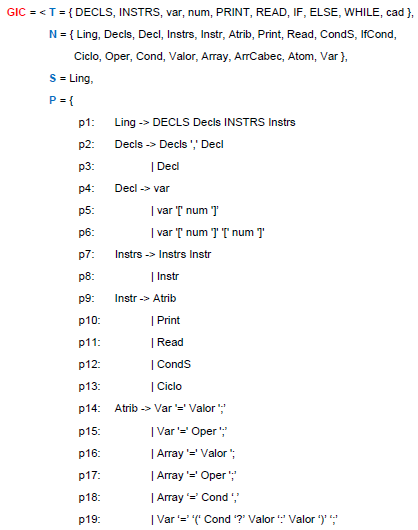
\includegraphics[width=120mm, scale=0.5]{gic1.PNG}
\end{figure}

\begin{figure}[h]
\centering
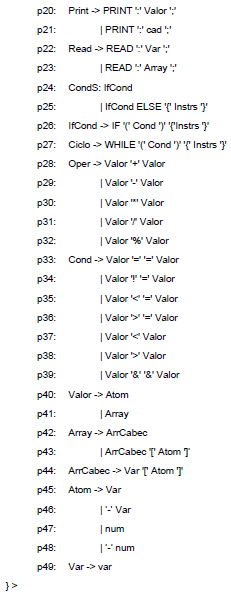
\includegraphics[width=80mm, scale=0.5]{gic2.PNG}
\end{figure}

%\begin{figure}[h]
%\centering
%
\includegraphics[width=120mm, scale=0.5]{Menu-Principal.png}
%\caption{\label{fig:change}Menu Principal.}
%\end{figure}

\chapter{Gramática tradutora da LIPS} \
A gramática independente de contexto, explicitada na secção anterior, deu origem à gramática tradutora que aqui se apresenta. 
\section{Declaração de variáveis}
As variáveis só podem tomar letras minúsculas e, para verificar re-declaração ou uso de variáveis não declaradas, é usada uma tabela de Hash que contém as variáveis declaradas. É no parsing da declaração de variáveis que esta tabela é preenchida - ao inserir uma variável, caso esta já exista na tabela a compilação termina. A verificação do uso de variáveis não declaradas é feita ao compilar as instruções, em que se confirma se a variável encontrada existe na tabela de Hash. Em caso negativo, o parsing termina.\\
Uma vez que é necessário guardar memória para cada variável, definiu-se uma estrutura a ser guardada como valor na tabela de Hash para cada variável. Esta estrutura contém dois valores: a posição em relação ao endereço gp e o tamanho de cada linha da matriz, ou seja, o número de colunas (caso a variável seja uma matriz). Para distinguir a posição de cada variável definiu-se também uma variável global que é incrementada à medida que são declaradas variáveis (1 caso seja uma variável "simples", n caso seja um array unidimensional, em que n é o tamanho do array, e n*m no caso da matriz em que n e m são os números de linhas e colunas, respetivamente).
\section{Atribuições}
É possível atribuir a variáveis: valores, operações ou condições. É ainda possível recorrer a um operador ternário. A atribuição pode ser feita quer a variáveis simples, quer a posições de arrays. Importa mencionar que um valor é um número ou o valor de uma variável, enquanto que uma operação é uma soma, subtração, multiplicação ou divisão de dois valores. Pode ainda ser calculado o resto da divisão inteira entre dois valores. Por sua vez, uma condição é um teste de igualdade, desigualdade, superioridade, etc., entre dois valores. Pode ser ainda calculado o valor lógico E entre dois valores (multiplicando os dois valores).
\section{Escrita}
Em cada PRINT apenas pode ser imprimido um valor ou uma cadeia de caracteres (cad).
\section{Leitura}
A leitura de valores pode ser feita para variáveis simples ou posições de arrays.
\section{Controlo de fluxo}
Para permitir efetuar instruções de controlo de fluxo é necessário criar labels diferentes entre cada uma das instruções. Para isso criou-se um contador que incrementa sempre que se adicionar uma instrução condicional ou cíclica.\\
No entanto, com esta solução é possível distinguir as labels se apenas existirem instruções encadeadas, já que, se existir alguma instrução de controlo de fluxo aninhada, quando se imprimir a label que se encontra no final do bloco esta vai ter um valor diferente da que está no início do bloco.\\
Para que seja possível incluir instruções aninhadas, construiu-se uma stack (LIFO) que guarda as labels que ainda não foram concluídas. Assim, sempre que se imprimir a primeira label, inclui-se essa label na stack e incrementa-se o seu valor. Quando chegar à altura de imprimir a segunda label, retira-se o seu valor da stack, pois a variável global pode ter sido alterada entretanto.\\
Desta forma, no caso de uma instrução condicional coloca-se a instrução "jz labelI1" imediatamente depois de testar a condição, sendo I1 a variável global que contem o número da label, e coloca-se I1 na stack, incrementando-a.\\
Se não existir bloco ELSE coloca-se a instrução "labelI1:" depois de executar o bloco, sendo I o valor que está na cabeça da stack, retirando-o.\\
Caso haja um bloco ELSE inclui-se as instruções "jump labelI2" e "labelI1" a seguir ao bloco do IF e antes do bloco de instruções do ELSE, sendo I1 obtido da stack e I2 a variável global (como sempre esta variável é incrementada depois de colocada na stack). No final do bloco ELSE coloca-se a instrução "labelI2:" sendo I2 obtido da stack.
\item Nas instruções ciclicas, coloca-se a instrução "labelI1:" antes de testar a condição, sendo o I1 o valor obtido da variável global (sendo colocada na stack e incrementada de seguida). Imediatamente depois de calcular a condição de paragem é colocada a instrução "jz labelI2" (mais uma vez é colocada na stack e incrementada). No final das instruções pertencentes ao bloco WHILE são adicionadas as instruções "jump labelI1" e "labelI2:", onde I1 e I2 são obtidos da stack.
\section{Assembly da Máquina Virtual VM}
Para gerar o compilador, foram tomadas algumas decisões a nível do \textit{Assembly}, tais como: 
\begin{itemize}
\item A atribuição de um valor a uma variável consiste em colocar o valor no topo da stack e executar a instrução "storeg P", onde P é a posição (em relação ao registo gp) onde se encontra a variável. Para atribuir um valor a uma posição de um array ou de uma matriz, é necessário colocar o apontador da matriz e o índice da posição no topo da stack. Para isso executam-se as seguintes instruções:
\begin{multicols}{2}
\begin{itemize}
\item \textbf{ARRAY}
\item pushgp
\item pushi P
\item padd
\item pushi I
\end{itemize}
\columnbreak
\begin{itemize}
\item \textbf{MATRIZ}
\item pushgp
\item pushi P
\item padd
\item pushi I
\item push T
\item mul
\item push J
\item (onde P é a posição do inicio do array (ou da matriz), I é o indice (das linhas, no caso de uma matriz), T é o tamanho de cada linha (no caso de uma matriz) e J é o indice das colunas);
\item Nota: o cálculo da posição de uma matriz é: I*T+J.
\end{itemize}
\end{multicols}
De seguida coloca-se o valor a atribuir no topo da stack e executa-se a instrução "storen".
\item Para colocar um valor numérico no topo da stack executa-se a instrução "pushi V" sendo V o valor númerico. A colocação de um valor de uma variável no topo da stack consiste em executar a instrução "pushg P". Para colocar o valor de uma posição de um array ou de uma matriz no topo da stack executa-se as seguintes instruções:
\begin{multicols}{2}
\begin{itemize}
\item \textbf{ARRAY}
\item pushgp
\item pushi P
\item padd
\item pushi I
\item loadn
\end{itemize}
\columnbreak
\begin{itemize}
\item \textbf{MATRIZ}
\item pushgp
\item pushi P
\item padd
\item pushi I
\item push T
\item mul
\item push J
\item loadn
\end{itemize}
\end{multicols}
\item Imprimir um valor consiste em colocar o valor no topo da stack e exectuar a instrução "writei" de seguida, enquanto que para imprimir uma cadeia de caracteres é necessário fazer push da cadeia e executar o comando "writes".
\item Uma vez que a linguagem apenas suporta inteiros (excetuando o caso de imprimir cadeias de caracteres), a leitura do standard input é feita com a instrução "read" seguida da instrução "atoi". Para guardar o valor numa variável ou numa posição de um array ou de uma matriz, o procedimento é o mesmo das atribuições.
\item O cálculo de uma qualquer operação consiste em colocar dois valores no topo da stack e executar a instrução pretendida (add, sub, mul, div, mod). A atribuição do valor resultante a uma variável é feita tal como explicado anteriormente.
\item Calcular uma condição segue a mesma lógica do cálculo das operações, variando apenas nas instruções usadas (equal, equal not, infeq, supeq, inf, sup). É ainda possível calcular o valor lógico E usando a instrução "mul".
\item Para permitir efetuar instruções de controlo de fluxo é necessário criar labels diferentes entre cada uma das instruções. Para isso criou-se um contador que incrementa sempre que se adicionar uma instrução condicional ou cíclica.
No entanto com esta solução é possível distinguir as labels se apenas existirem instruções encadeadas, já que se existir alguma instrução de controlo de fluxo aninhada quando se imprimir a label que se encontra no final do bloco esta vai ter um valor diferente da que está no inicio do bloco.\\
Para que seja possível incluir instruções aninhadas construiu-se uma stack (LIFO) que guarda as labels que ainda não foram concluídas. Assim, sempre que se imprimir a primeira label, inclui-se essa label na stack e incrementa-se o seu valor. Quando chegar à altura de imprimir a segunda label retira-se o seu valor da stack, pois a variável global pode ter sido alterada entrentanto.\\
Desta forma, no caso de uma instrução condicional coloca-se a instrução "jz labelI1" imediatamente depois de testar a condição, sendo I1 a variável global que contem o número da label, e coloca-se I1 na stack, incrementando-a. 
Se não existir bloco ELSE coloca-se a instrução "labelI1:" depois de executar o bloco, sendo I o valor que está na cabeça da stack, retirando-o.\\
Caso haja um bloco ELSE inclui-se as instruções "jump labelI2" e "labelI1" a seguir ao bloco do IF e antes do bloco de instruções do ELSE, sendo I1 obtido da stack e I2 a variável global (como sempre esta variável é incrementada depois decolocada na stack). No final do bloco ELSE coloca-se a instrução "labelI2:" sendo I2 obtido da stack.
\item Nas instruções ciclicas, coloca-se a instrução "labelI1:" antes de testar a condição, sendo o I1 o valor obtido da variável global (sendo colocada na stack e incrementada de seguida). Imediatamente depois de calcular a condição de paragem é colocada a instrução "jz labelI2" (mais uma vez é colocada na stack e incrementada). No final das instruções pertencentes ao bloco WHILE são adicionadas as instruções "jump labelI1" e "labelI2:", onde I1 e I2 são obtidos da stack.\\\\ 
\textbf{NOTAS:}\\
Nas produções relativas aos não terminais CondS e Array numa primeira abordagem colocou-se as seguintes produções:
\begin{verbatim}
CondS: IF '(' Cond ')' { fprintf(f, "\tjz label%d\n", label); push(); }
	   '{' Instrs '}' { fprintf(f, "label%d:\n", pop()); }

     | IF '(' Cond ')' { fprintf(f, "\tjz label%d\n", label); push(); }
       '{' Instrs '}' ELSE { fprintf(f, "\tjump label%d\n", label);
     			  		     fprintf(f, "label%d:\n", pop()); 
   						     push(); } '{' Instrs '}' { fprintf(f, "label%d:\n", pop()); }

Array: Var {fprintf(f, "\tpushgp\n\tpushi %d\n\tpadd\n", $1.pos);} '[' Atom ']'

     | Var {fprintf(f, "\tpushgp\n\tpushi %d\n\tpadd\n", $1.pos);} '[' Atom ']'
           { fprintf(f, "\tpushi %d\n\tmul\n", $1.tamL);} '[' Atom ']' {fprintf(f, "\tadd\n"); }
\end{verbatim}
Uma vez que esta abordagem gerava conflitos passou-se as partes iniciais que eram comuns às duas alternativas de cada não terminal para uma outra produção. Desta forma eliminou-se os conflitos.\\\\\\\\\\
\end{itemize}
\section{Exposição da GT}
\begin{figure}[ht]
\centering
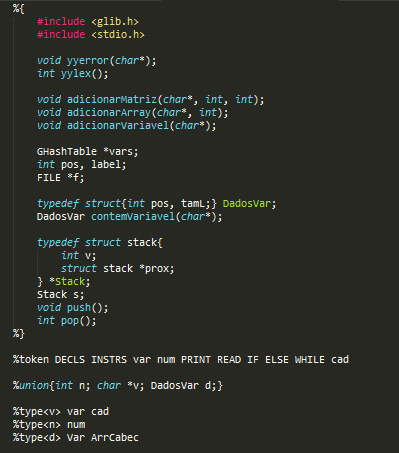
\includegraphics[width=80mm, scale=0.5]{gt1.png}
\caption{\label{fig:change}Declarações e estruturas de dados.}
\end{figure}

\begin{figure}[ht]
\centering
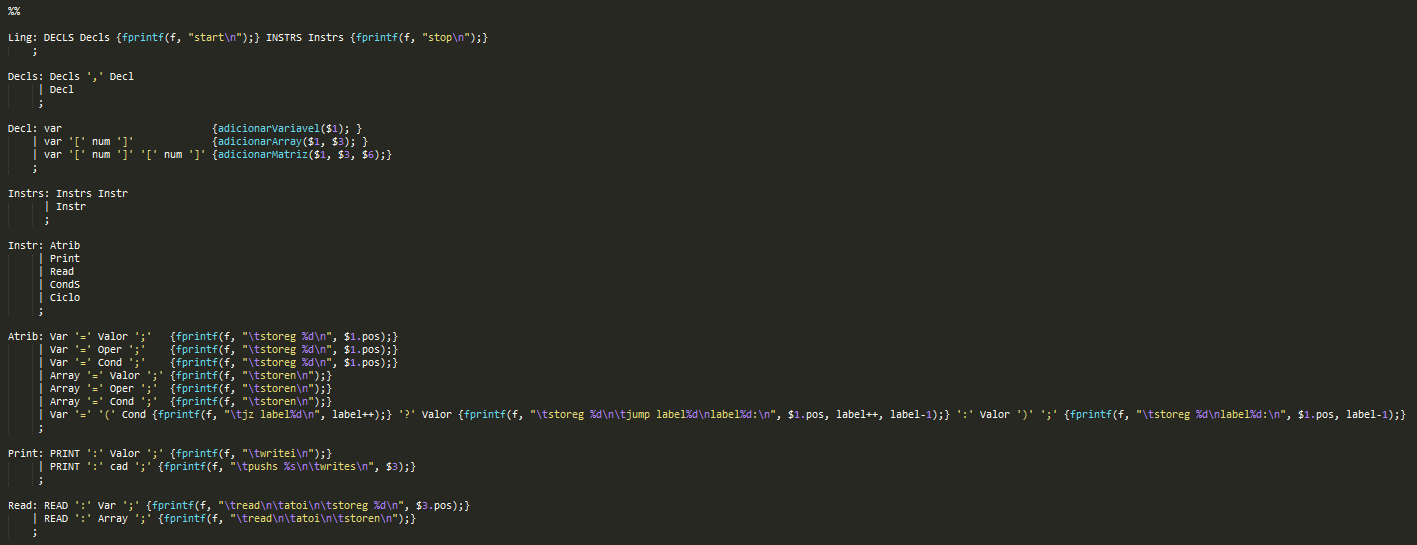
\includegraphics[width=180mm, scale=0.9]{gt2.PNG}
\caption{\label{fig:change}Gramática tradutora (1).}
\end{figure}

\begin{figure}[ht]
\centering
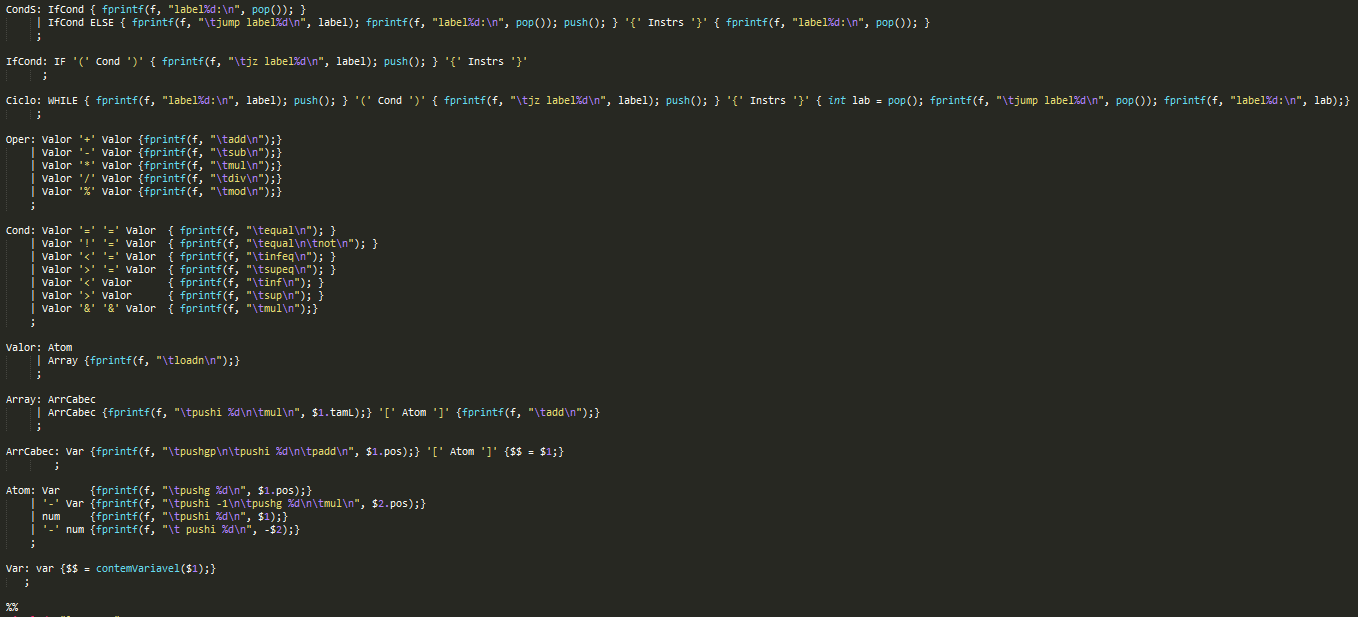
\includegraphics[width=180mm, scale=0.9]{gt3.PNG}
\caption{\label{fig:change}Gramática tradutora (2).}
\end{figure}

\begin{figure}[ht]
\centering
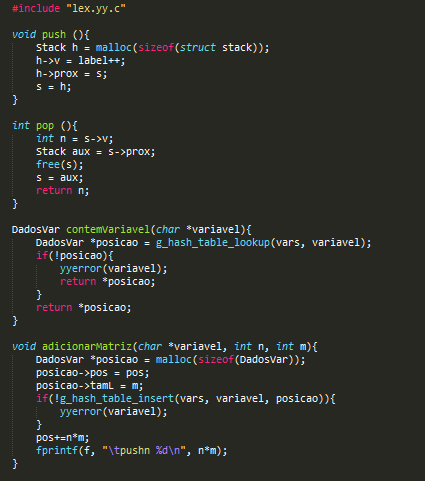
\includegraphics[width=80mm, scale=0.5]{gt4.png}
\caption{\label{fig:change}Funções auxiliares criadas.}
\end{figure}

\begin{figure}[ht]
\centering
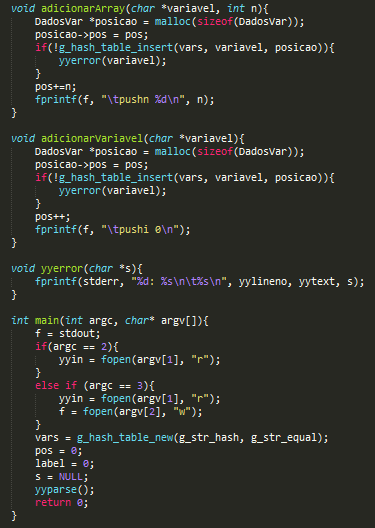
\includegraphics[width=80mm, scale=0.5]{gt5.png}
\caption{\label{fig:change}Funções auxiliares e main.}
\end{figure}

\section{Analisador léxico da gramática}
\begin{figure}[ht]
\centering
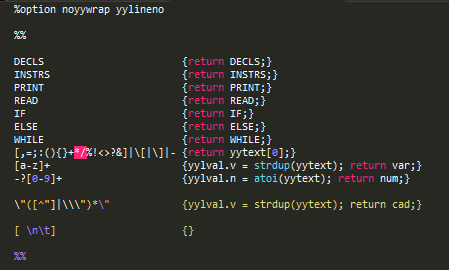
\includegraphics[width=100mm, scale=0.5]{flex.png}
\end{figure}

\chapter{Apresentação de exemplos de utilização}
A extensão escolhida para a LPIS foi \textit{.ex}.\\
O enunciado do projeto propõe a apresentação de seis exemplos, que se mencionam a seguir juntamente com a sua resolução em LPIS:
\begin{itemize}
	\item ler 4 números e dizer se podem ser os lados de um quadrado:
	\begin{figure}[h]
	\centering
	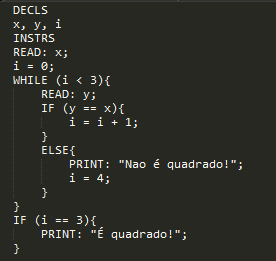
\includegraphics[width=60mm, scale=0.5]{ex1.PNG}
	\end{figure}
	\newpage
	\item ler um inteiro N, depois ler N números e escrever o menor deles:
	\begin{figure}[h]
	\centering
	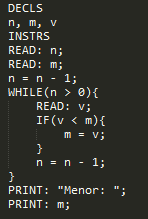
\includegraphics[width=50mm, scale=0.5]{ex2.PNG}
	\end{figure}
	\item ler N (constante do programa) números e calcular e imprimir o seu produtório:
	\begin{figure}[h]
	\centering
	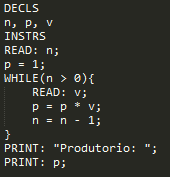
\includegraphics[width=50mm, scale=0.5]{ex3.PNG}
	\end{figure}
	\newpage
	\item contar e imprimir os números impares de uma sequência de números naturais:
	\begin{figure}[h]
	\centering
	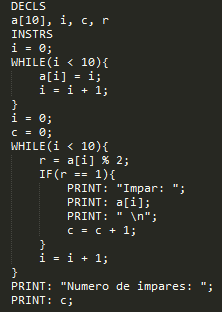
\includegraphics[width=50mm, scale=0.5]{ex4.PNG}
	\end{figure}
	\item ler e armazenar os elementos de um vetor de comprimento N; imprimir os valores por ordem decrescente após fazer a ordenação do array por trocas diretas:
	\begin{figure}[h]
	\centering
	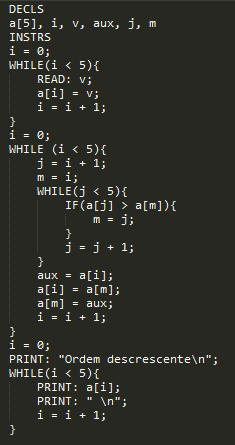
\includegraphics[width=50mm, scale=0.5]{ex5.PNG}
	\end{figure}
	\newpage
	\item ler e armazenar N números num array; imprimir os valores por ordem inversa:
	\begin{figure}[h]
	\centering
	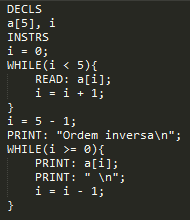
\includegraphics[width=50mm, scale=0.5]{ex6.PNG}
	\end{figure}
\end{itemize}


\chapter{Conclusão} \label{concl}
Concluído o projeto, destaca-se o sucesso na criação de uma linguagem de programação imperativa simples que faculta funcionalidades para a obtenção dos resultados pretendidos nos programas sugeridos no enunciado.\\
Este trabalho foi importante para cimentar os conhecimentos sobre YACC e FLEX, bem como relembrar conhecimentos sobre análise de código em linguagem máquina \textit{Assembly} e posterior implementação nesta mesma linguagem.\\
Quanto a trabalho futuro, seria lógico tentar estender a linguagem de forma a esta ficar mais completa, sendo possível outros tipos de dados e não apenas inteiros, ser possível a criação de estruturas de dados, entre outras que são conhecidas das linguagens de programação imperativas mais conhecidas.


\end{document} 